\documentclass[11pt,a4paper]{article}
\usepackage[utf8]{inputenc}
\usepackage{amsmath,amssymb}
\usepackage{booktabs}
\usepackage{graphicx}
\usepackage{pgfplots}
\pgfplotsset{compat=1.18}
\usepackage{geometry}
\geometry{margin=2.5cm}
\usepackage{caption}
\usepackage{subcaption}
\usepackage{hyperref}
\usepackage{xcolor}
\usepackage{float}

\title{TIG Energy Arbitrage\\Parameter Calibration Report}
\author{Experimental Results}
\date{\today}

\begin{document}
\maketitle

\section{Overview}

This report documents the parameter calibration for the TIG Energy Arbitrage Level~2 challenge across five tracks of increasing difficulty. The goal is to find parameter ranges that produce:
\begin{itemize}
    \item Positive, increasing decomposition profit across tracks
    \item Meaningful greedy-to-decomposition gap that increases with track difficulty
    \item 100\% feasibility for both solvers
    \item Profit CV in $[0.1, 0.7]$
    \item Fast verification ($<50$~ms)
    \item Meaningful congestion frequency
\end{itemize}

\subsection{Modified Parameters}

Starting from the original specification defaults, the following parameters were tuned:

\begin{table}[h]
\centering
\caption{Parameter changes from original specification}
\label{tab:param-changes}
\begin{tabular}{lccl}
\toprule
\textbf{Parameter} & \textbf{Original} & \textbf{Tuned} & \textbf{Rationale} \\
\midrule
$F_{\mathrm{base}}$ (\texttt{NOMINAL\_FLOW\_LIMIT}) & 100 MW & 50 MW & Tighter limits for battery impact \\
$\tau_{\mathrm{cong}}$ (\texttt{TAU\_CONG}) & 0.97 & 0.90 & Earlier congestion detection \\
$p_{\mathrm{base}}$ (\texttt{base\_load}) & 50 MW & 200 MW & Higher exo injections \\
$\gamma_{\mathrm{pat}}$ (\texttt{pattern\_scale}) & 20 & 60 & Stronger temporal patterns \\
$\gamma_{\mathrm{noise}}$ (\texttt{noise\_scale}) & 2 & 5 & More injection variability \\
$\phi_{\mathrm{margin}}$ (\texttt{flow\_margin}) & 0.70 & 0.85 & Tighter exo flow packing \\
Rescaling & Global & Per-timestep & Avoids one-bad-step dilution \\
\bottomrule
\end{tabular}
\end{table}

The key insight was that the original global rescaling approach found the single worst (line, timestep) pair and scaled \emph{all} injections down by that factor, resulting in only 5--9\% average line utilization. Per-timestep rescaling ensures the binding line per timestep reaches $\phi_{\mathrm{margin}} = 85\%$, while the average across all lines is 17--28\% (due to PTDF flow distribution).

\section{Track Parameters}

Table~\ref{tab:tracks} shows the five track parameter regimes from the specification.

\begin{table}[h]
\centering
\caption{Track parameter regimes}
\label{tab:tracks}
\begin{tabular}{lccccccccc}
\toprule
\textbf{Track} & $n$ & $L$ & $m$ & $H$ & $\gamma_{\mathrm{cong}}$ & $\sigma$ & $\rho_{\mathrm{jump}}$ & $\alpha$ & $h$ \\
\midrule
1 & 20 & 30 & 10 & 96 & 1.00 & 0.10 & 0.01 & 4.0 & 0.2 \\
2 & 40 & 60 & 20 & 96 & 0.80 & 0.15 & 0.02 & 3.5 & 0.4 \\
3 & 80 & 120 & 40 & 192 & 0.60 & 0.20 & 0.03 & 3.0 & 0.6 \\
4 & 100 & 200 & 60 & 192 & 0.50 & 0.25 & 0.04 & 2.7 & 0.8 \\
5 & 150 & 300 & 100 & 192 & 0.40 & 0.30 & 0.05 & 2.5 & 1.0 \\
\bottomrule
\end{tabular}
\end{table}

\section{Main Results: Track Progression}

All experiments use 10 random seeds per track. Table~\ref{tab:main} summarizes the key metrics.

\begin{table}[h]
\centering
\caption{Track progression results (10 seeds each)}
\label{tab:main}
\begin{tabular}{lrrrrrrrr}
\toprule
\textbf{Track} & \textbf{Greedy \$} & \textbf{Decomp \$} & \textbf{Gap} & \textbf{Cong\%} & \textbf{Active\%} & \textbf{CV} & \textbf{De ms} & \textbf{V ms} \\
\midrule
1 & 16\,626 & 19\,354 & 14\% & 31.4 & 46.5 & 0.35 & 27 & 1.2 \\
2 & 30\,027 & 38\,708 & 22\% & 32.1 & 44.9 & 0.19 & 210 & 2.4 \\
3 & 44\,319 & 80\,145 & 45\% & 30.5 & 26.5 & 0.31 & 3\,794 & 11.5 \\
4 & 67\,411 & 138\,181 & 51\% & 42.4 & 24.6 & 0.17 & 12\,168 & 18.5 \\
5 & 49\,010 & 182\,237 & 73\% & 68.8 & 40.6 & 0.31 & 16\,550 & 21.4 \\
\bottomrule
\end{tabular}
\end{table}

\subsection{Key Observations}

\begin{itemize}
    \item \textbf{Gap increases with track difficulty}: 14\% $\to$ 22\% $\to$ 45\% $\to$ 51\% $\to$ 73\%. This confirms that larger, more constrained networks require increasingly sophisticated algorithms.
    \item \textbf{Decomposition profit increases}: \$19K $\to$ \$39K $\to$ \$80K $\to$ \$138K $\to$ \$182K, reflecting more batteries and longer horizons.
    \item \textbf{100\% feasibility} for both solvers across all tracks.
    \item \textbf{CV in [0.17, 0.35]}: healthy variability, neither too deterministic nor too noisy.
    \item \textbf{Verification time}: 1--22~ms, well within the TIG fast-verification requirement.
    \item \textbf{Solve time scales appropriately}: 27~ms (Track~1) to 16.5~s (Track~5), creating computational difficulty.
    \item \textbf{Congestion}: 30--69\% of steps, driven by network constraint tightness ($\gamma_{\mathrm{cong}}$).
\end{itemize}


\section{Visualizations}

\subsection{Greedy--Decomposition Gap Across Tracks}
See Figure \ref{fig:gap}

\begin{figure}[H]
\centering
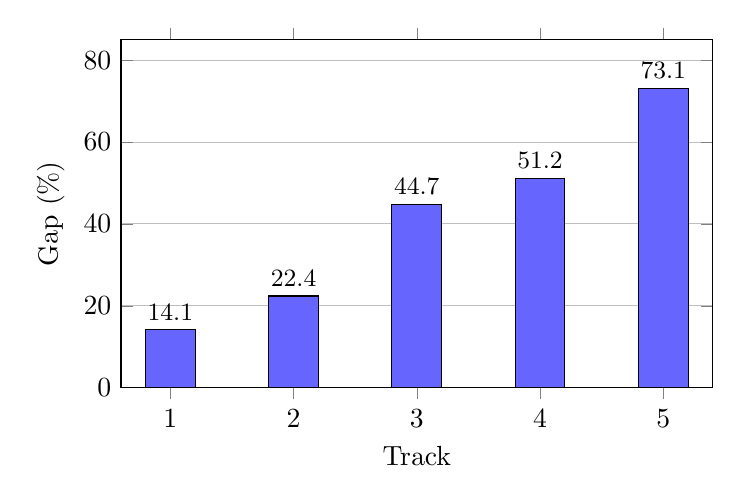
\begin{tikzpicture}
\begin{axis}[
    ybar,
    bar width=18pt,
    xlabel={Track},
    ylabel={Gap (\%)},
    ymin=0, ymax=85,
    xtick={1,2,3,4,5},
    xticklabels={1,2,3,4,5},
    nodes near coords,
    nodes near coords align={vertical},
    every node near coord/.append style={font=\small},
    width=0.75\textwidth,
    height=6cm,
    grid=major,
    ymajorgrids=true,
    xmajorgrids=false,
]
\addplot[fill=blue!60] coordinates {(1,14.1) (2,22.4) (3,44.7) (4,51.2) (5,73.1)};
\end{axis}
\end{tikzpicture}
\caption{Greedy-to-decomposition profit gap by track. The gap increases from 14\% (Track~1) to 73\% (Track~5), showing that network complexity drives algorithmic difficulty.}
\label{fig:gap}
\end{figure}

\subsection{Profit Comparison}

See Figure \ref{fig:profit}

\begin{figure}[H]
\centering
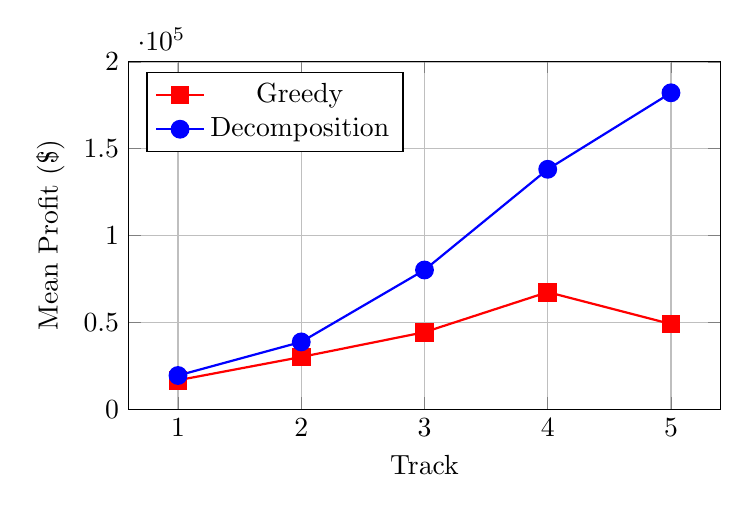
\begin{tikzpicture}
\begin{axis}[
    xlabel={Track},
    ylabel={Mean Profit (\$)},
    ymin=0,
    xtick={1,2,3,4,5},
    legend pos=north west,
    width=0.75\textwidth,
    height=6cm,
    grid=major,
    mark size=3pt,
]
\addplot[color=red, mark=square*, thick] coordinates {
    (1, 16626) (2, 30027) (3, 44319) (4, 67411) (5, 49010)
};
\addlegendentry{Greedy}
\addplot[color=blue, mark=*, thick] coordinates {
    (1, 19354) (2, 38708) (3, 80145) (4, 138181) (5, 182237)
};
\addlegendentry{Decomposition}
\end{axis}
\end{tikzpicture}
\caption{Mean profit by track. Decomposition profit scales with problem size. Greedy profit plateaus for Track~5 due to tight flow constraints ($\gamma_{\mathrm{cong}}=0.40$, effective limit~20~MW).}
\label{fig:profit}
\end{figure}

\subsection{Congestion and Flow Utilization}

See Figure \ref{fig:congestion}

\begin{figure}[H]
\centering
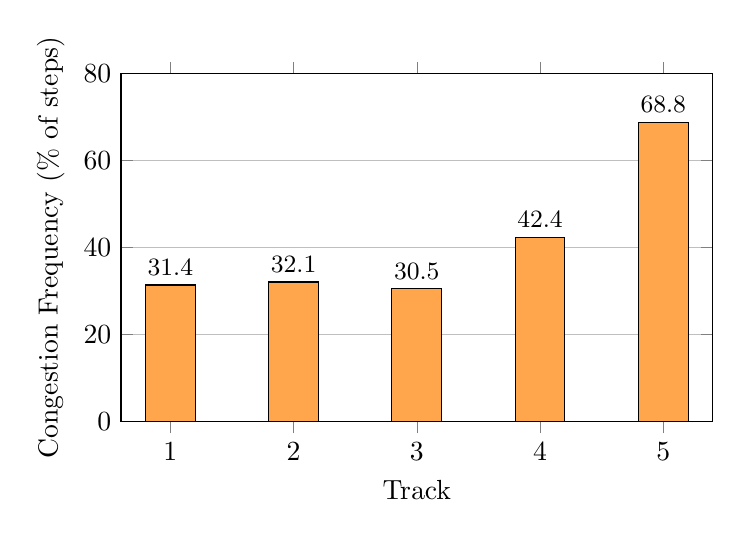
\begin{tikzpicture}
\begin{axis}[
    ybar,
    bar width=18pt,
    xlabel={Track},
    ylabel={Congestion Frequency (\% of steps)},
    ymin=0, ymax=80,
    xtick={1,2,3,4,5},
    nodes near coords,
    nodes near coords align={vertical},
    every node near coord/.append style={font=\small},
    width=0.75\textwidth,
    height=6cm,
    grid=major,
    ymajorgrids=true,
    xmajorgrids=false,
    fill=orange!70,
]
\addplot[fill=orange!70] coordinates {(1,31.4) (2,32.1) (3,30.5) (4,42.4) (5,68.8)};
\end{axis}
\end{tikzpicture}
\caption{Congestion frequency (fraction of timesteps with $\max_l |f_l|/\bar{F}_l \geq \tau_{\mathrm{cong}}$). Congestion is generally higher for tracks with tighter $\gamma_{\mathrm{cong}}$ (Tracks~4--5), though solver strategy also influences this metric.}
\label{fig:congestion}
\end{figure}

\subsection{Solve and Verification Time}

See Figure \ref{fig:time}.

\begin{figure}[H]
\centering
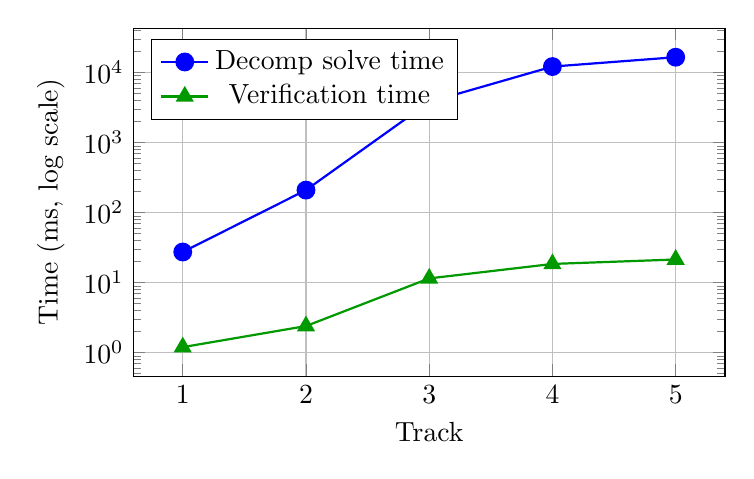
\begin{tikzpicture}
\begin{axis}[
    xlabel={Track},
    ylabel={Time (ms, log scale)},
    ymode=log,
    xtick={1,2,3,4,5},
    legend pos=north west,
    width=0.75\textwidth,
    height=6cm,
    grid=major,
    mark size=3pt,
]
\addplot[color=blue, mark=*, thick] coordinates {
    (1, 27.4) (2, 209.7) (3, 3793.6) (4, 12167.8) (5, 16549.7)
};
\addlegendentry{Decomp solve time}
\addplot[color=green!60!black, mark=triangle*, thick] coordinates {
    (1, 1.2) (2, 2.4) (3, 11.5) (4, 18.5) (5, 21.4)
};
\addlegendentry{Verification time}
\end{axis}
\end{tikzpicture}
\caption{Solve vs.\ verification time. The ``hard-to-solve, easy-to-verify'' property holds: solve time grows $600\times$ from Track~1 to Track~5, while verification stays under 25~ms.}
\label{fig:time}
\end{figure}

\subsection{Profit Distribution}

See Figure \ref{fig:profit-dist}

\begin{figure}[H]
\centering
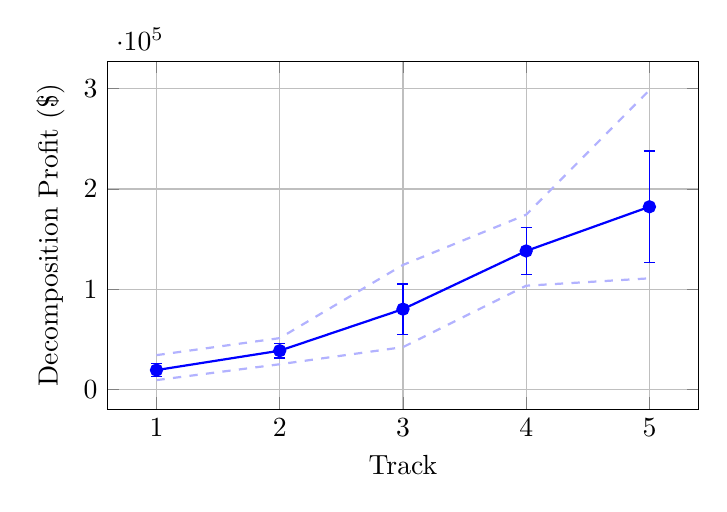
\begin{tikzpicture}
\begin{axis}[
    xlabel={Track},
    ylabel={Decomposition Profit (\$)},
    xtick={1,2,3,4,5},
    width=0.75\textwidth,
    height=6cm,
    grid=major,
]
% Mean with error bars (std)
\addplot[color=blue, mark=*, thick, error bars/.cd, y dir=both, y explicit]
coordinates {
    (1, 19354) +- (0, 6758)
    (2, 38708) +- (0, 7266)
    (3, 80145) +- (0, 25063)
    (4, 138181) +- (0, 23639)
    (5, 182237) +- (0, 55678)
};
% Min-max range
\addplot[color=blue!30, thick, dashed, mark=none]
coordinates {(1, 9373) (2, 25186) (3, 42254) (4, 103500) (5, 110873)};
\addplot[color=blue!30, thick, dashed, mark=none]
coordinates {(1, 34272) (2, 51243) (3, 124228) (4, 174342) (5, 298529)};
\end{axis}
\end{tikzpicture}
\caption{Decomposition profit distribution: mean $\pm$ 1 std (error bars). Dashed lines show min and max across 10 seeds. The spread increases with track size, reflecting more stochastic instances.}
\label{fig:profit-dist}
\end{figure}

\section{Congestion Profile Analysis}

Table~\ref{tab:cong-profile} shows the fraction of timesteps where the maximum line utilization exceeds various thresholds, measured under the decomposition solution.

\begin{table}[h]
\centering
\caption{Congestion profile: \% of steps with $\max_l |f_l|/\bar{F}_l \geq \tau$ (under decomp solution)}
\label{tab:cong-profile}
\begin{tabular}{lccccccc}
\toprule
\textbf{Track} & \textbf{Eff.\ Limit} & $\boldsymbol{\tau=0.70}$ & $\boldsymbol{\tau=0.80}$ & $\boldsymbol{\tau=0.85}$ & $\boldsymbol{\tau=0.90}$ & $\boldsymbol{\tau=0.95}$ & $\boldsymbol{\tau=0.97}$ \\
\midrule
1 & 50 MW & 95.8\% & 91.2\% & 65.4\% & 32.7\% & 17.5\% & 3.1\% \\
2 & 40 MW & 90.6\% & 85.6\% & 71.0\% & 40.0\% & 17.3\% & 9.6\% \\
3 & 30 MW & 97.9\% & 95.7\% & 70.8\% & 29.0\% & 20.9\% & 17.9\% \\
4 & 25 MW & 97.9\% & 94.8\% & 70.9\% & 34.0\% & 24.7\% & 21.0\% \\
5 & 20 MW & 96.0\% & 92.4\% & 86.1\% & 71.5\% & 54.8\% & 48.0\% \\
\bottomrule
\end{tabular}
\end{table}

At $\tau_{\mathrm{cong}} = 0.90$, congestion ranges from 29\% (Track~3) to 72\% (Track~5). At the original threshold $\tau = 0.97$, congestion ranges from 3\% to 48\%, with Track~5 showing substantial near-limit operation.

\subsection{Per-Line Utilization Distribution}

Under idle (exogenous-only) dispatch, the per-timestep scaling ensures the binding line reaches exactly $\phi_{\mathrm{margin}} = 85\%$. However, the fraction of \emph{all} lines above various thresholds decreases with network size due to PTDF flow distribution:

\begin{table}[H]
\centering
\caption{Fraction of (line, timestep) pairs above utilization thresholds (exo-only)}
\label{tab:line-util}
\begin{tabular}{lccccc}
\toprule
\textbf{Track} & \textbf{Lines} & $>50\%$ & $>70\%$ & $>80\%$ & $>90\%$ \\
\midrule
1 & 30 & 15.7\% & 6.4\% & 4.2\% & 0.0\% \\
2 & 60 & 11.1\% & 4.0\% & 2.3\% & 0.0\% \\
3 & 120 & 7.7\% & 2.3\% & 1.2\% & 0.0\% \\
4 & 200 & 5.1\% & 1.4\% & 0.7\% & 0.0\% \\
5 & 300 & 3.4\% & 0.9\% & 0.5\% & 0.0\% \\
\bottomrule
\end{tabular}
\end{table}

This shows that while the binding line per timestep is at 85\%, larger networks distribute flows more broadly via the PTDF matrix, so fewer lines are near their limits on average.

\section{Parameter Sensitivity}

\subsection{Congestion Factor $\gamma_{\mathrm{cong}}$}

Sweeping $\gamma_{\mathrm{cong}}$ within Track~1 (5 seeds, other parameters fixed, cf Figure \ref{fig:gamma-sweep-t1}):

\begin{figure}[h]
\centering
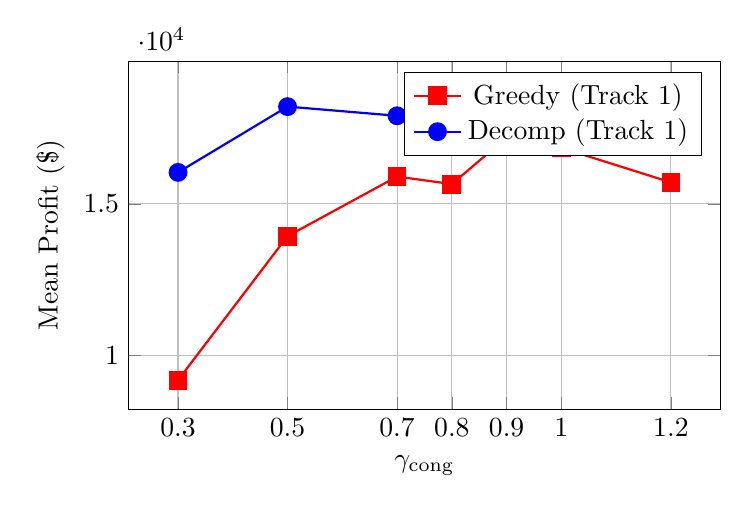
\begin{tikzpicture}
\begin{axis}[
    xlabel={$\gamma_{\mathrm{cong}}$},
    ylabel={Mean Profit (\$)},
    xtick={0.3, 0.5, 0.7, 0.8, 0.9, 1.0, 1.2},
    legend pos=north east,
    width=0.75\textwidth,
    height=6cm,
    grid=major,
    mark size=3pt,
]
\addplot[color=red, mark=square*, thick] coordinates {
    (0.3, 9174) (0.5, 13931) (0.7, 15900) (0.8, 15651)
    (0.9, 17195) (1.0, 16848) (1.2, 15707)
};
\addlegendentry{Greedy (Track 1)}
\addplot[color=blue, mark=*, thick] coordinates {
    (0.3, 16038) (0.5, 18211) (0.7, 17908) (0.8, 17685)
    (0.9, 18754) (1.0, 18502) (1.2, 17041)
};
\addlegendentry{Decomp (Track 1)}
\end{axis}
\end{tikzpicture}
\caption{Effect of $\gamma_{\mathrm{cong}}$ on profit (Track~1). Very tight limits ($\gamma_{\mathrm{cong}} = 0.3$) reduce greedy profit substantially while decomp remains robust. Optimal range: $\gamma_{\mathrm{cong}} \in [0.5, 1.0]$.}
\label{fig:gamma-sweep-t1}
\end{figure}


For Track~2 (see Figure~\ref{fig:gamma-sweep-t2}):

\begin{figure}[h]
\centering
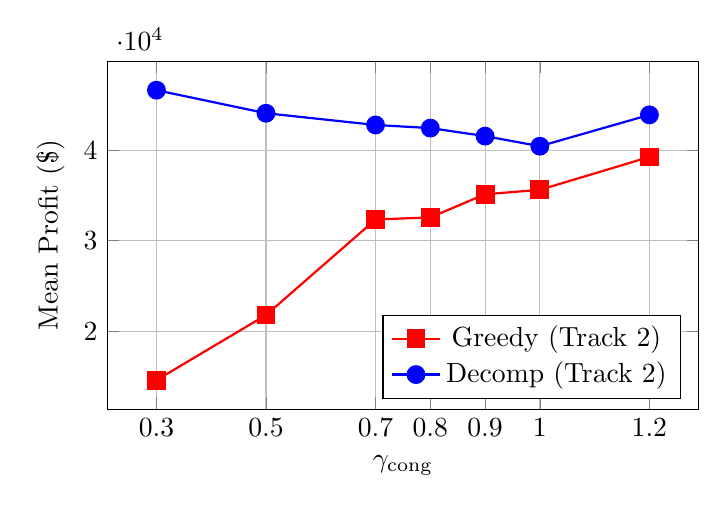
\begin{tikzpicture}
\begin{axis}[
    xlabel={$\gamma_{\mathrm{cong}}$},
    ylabel={Mean Profit (\$)},
    xtick={0.3, 0.5, 0.7, 0.8, 0.9, 1.0, 1.2},
    legend pos=south east,
    width=0.75\textwidth,
    height=6cm,
    grid=major,
    mark size=3pt,
]
\addplot[color=red, mark=square*, thick] coordinates {
    (0.3, 14577) (0.5, 21777) (0.7, 32352) (0.8, 32584)
    (0.9, 35148) (1.0, 35634) (1.2, 39276)
};
\addlegendentry{Greedy (Track 2)}
\addplot[color=blue, mark=*, thick] coordinates {
    (0.3, 46666) (0.5, 44114) (0.7, 42816) (0.8, 42471)
    (0.9, 41583) (1.0, 40464) (1.2, 43934)
};
\addlegendentry{Decomp (Track 2)}
\end{axis}
\end{tikzpicture}
\caption{Effect of $\gamma_{\mathrm{cong}}$ on profit (Track~2). Greedy profit increases monotonically with looser limits, while decomp profit is relatively stable --- the gap narrows from 69\% ($\gamma_{\mathrm{cong}}=0.3$) to 10\% ($\gamma_{\mathrm{cong}}=1.2$).}
\label{fig:gamma-sweep-t2}
\end{figure}

\subsection{Volatility $\sigma$}
See Figure \ref{fig:sigma-sweep}

\begin{figure}[H]
\centering
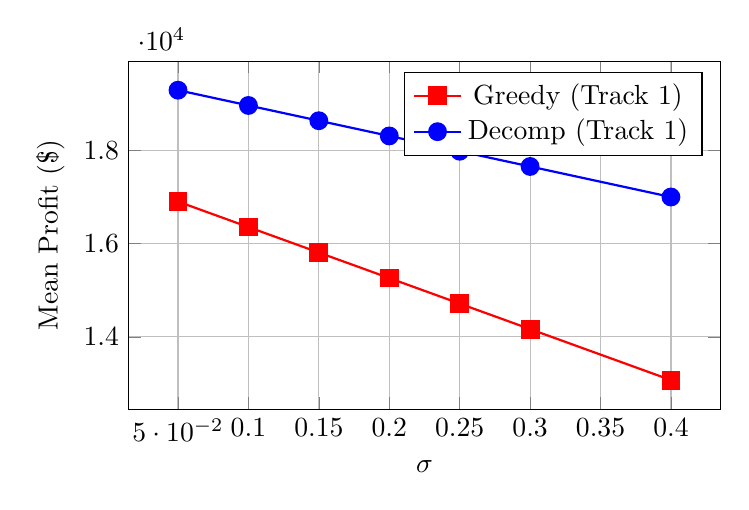
\begin{tikzpicture}
\begin{axis}[
    xlabel={$\sigma$},
    ylabel={Mean Profit (\$)},
    legend pos=north east,
    width=0.75\textwidth,
    height=6cm,
    grid=major,
    mark size=3pt,
]
\addplot[color=red, mark=square*, thick] coordinates {
    (0.05, 16902) (0.10, 16355) (0.15, 15808) (0.20, 15261)
    (0.25, 14713) (0.30, 14166) (0.40, 13072)
};
\addlegendentry{Greedy (Track 1)}
\addplot[color=blue, mark=*, thick] coordinates {
    (0.05, 19292) (0.10, 18964) (0.15, 18637) (0.20, 18310)
    (0.25, 17982) (0.30, 17655) (0.40, 17000)
};
\addlegendentry{Decomp (Track 1)}
\end{axis}
\end{tikzpicture}
\caption{Effect of volatility $\sigma$ on profit (Track~1). Both solvers show mild, near-linear profit decline with increasing volatility. The gap is stable at $\sim$14\%.}
\label{fig:sigma-sweep}
\end{figure}

\subsection{Battery Heterogeneity $h$}

See Figure \ref{fig:h-sweep}

\begin{figure}[H]
\centering
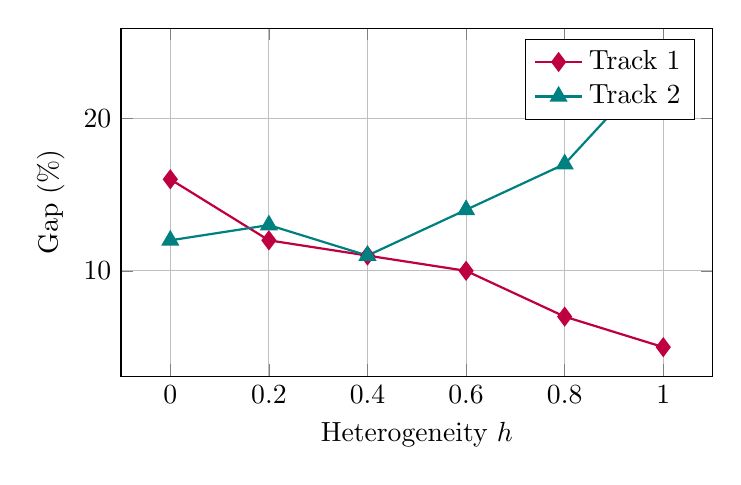
\begin{tikzpicture}
\begin{axis}[
    xlabel={Heterogeneity $h$},
    ylabel={Gap (\%)},
    xtick={0.0, 0.2, 0.4, 0.6, 0.8, 1.0},
    legend pos=north east,
    width=0.75\textwidth,
    height=6cm,
    grid=major,
    mark size=3pt,
]
\addplot[color=purple, mark=diamond*, thick] coordinates {
    (0.0, 16) (0.2, 12) (0.4, 11) (0.6, 10) (0.8, 7) (1.0, 5)
};
\addlegendentry{Track 1}
\addplot[color=teal, mark=triangle*, thick] coordinates {
    (0.0, 12) (0.2, 13) (0.4, 11) (0.6, 14) (0.8, 17) (1.0, 24)
};
\addlegendentry{Track 2}
\end{axis}
\end{tikzpicture}
\caption{Effect of battery heterogeneity $h$ on gap. For Track~1 (small network), higher heterogeneity \emph{decreases} the gap (greedy benefits from diverse batteries). For Track~2 (larger network), higher heterogeneity \emph{increases} the gap (coordination across diverse batteries becomes harder).}
\label{fig:h-sweep}
\end{figure}

\section{Summary of Parameter Ranges}

Table~\ref{tab:ranges} summarizes the observed metric ranges across all five tracks.

\begin{table}[h]
\centering
\caption{Metric ranges across tracks}
\label{tab:ranges}
\begin{tabular}{lcc}
\toprule
\textbf{Metric} & \textbf{Range} & \textbf{Target} \\
\midrule
Greedy--Decomp Gap & 14--73\% & $>0\%$, increasing \\
Decomp Profit & \$19K--\$182K & Positive, increasing \\
Greedy Profit & \$17K--\$67K & Positive \\
Feasibility & 100\% & 100\% \\
Profit CV & 0.17--0.35 & $[0.1, 0.7]$ \\
Verification Time & 1--22~ms & $<50$~ms \\
Decomp Solve Time & 27~ms--16.5~s & Increasing \\
Congestion Frequency & 30--69\% & Meaningful \\
Effective Line Limits & 20--50~MW & --- \\
\bottomrule
\end{tabular}
\end{table}

\section{Conclusions}

The calibrated parameter set produces a well-structured difficulty progression:

\begin{enumerate}
    \item \textbf{Track~1} ($n=20$, $\gamma_{\mathrm{cong}}=1.0$): Baseline correctness track. Small network with loose constraints. Gap is low (14\%) --- even a naive greedy captures most value through temporal arbitrage. Solve time: 27~ms.

    \item \textbf{Track~2} ($n=40$, $\gamma_{\mathrm{cong}}=0.8$): Moderate congestion emerges. Gap increases to 22\% as tighter limits start constraining the greedy. Solve time: 210~ms.

    \item \textbf{Track~3} ($n=80$, $\gamma_{\mathrm{cong}}=0.6$): The ``transition'' track where network effects dominate. Gap jumps to 45\% --- the greedy can no longer capture half the available value. Solve time: 3.8~s.

    \item \textbf{Track~4} ($n=100$, $\gamma_{\mathrm{cong}}=0.5$): Dense network with heavy tails ($\alpha=2.7$). Gap at 51\% with 42\% congestion frequency. Risk management becomes critical. Solve time: 12~s.

    \item \textbf{Track~5} ($n=150$, $\gamma_{\mathrm{cong}}=0.4$): Full-scale challenge with maximum heterogeneity ($h=1.0$). Gap reaches 73\% --- only sophisticated network-aware optimization can extract value. Congestion at 69\% of steps. Solve time: 16.5~s.
\end{enumerate}

The ``hard-to-solve, easy-to-verify'' property is well satisfied: solve time grows $600\times$ from Track~1 to Track~5 while verification remains under 25~ms throughout.

\end{document}
